
\label{sec:beam}
\begin{figure}[ht]
    \centering
    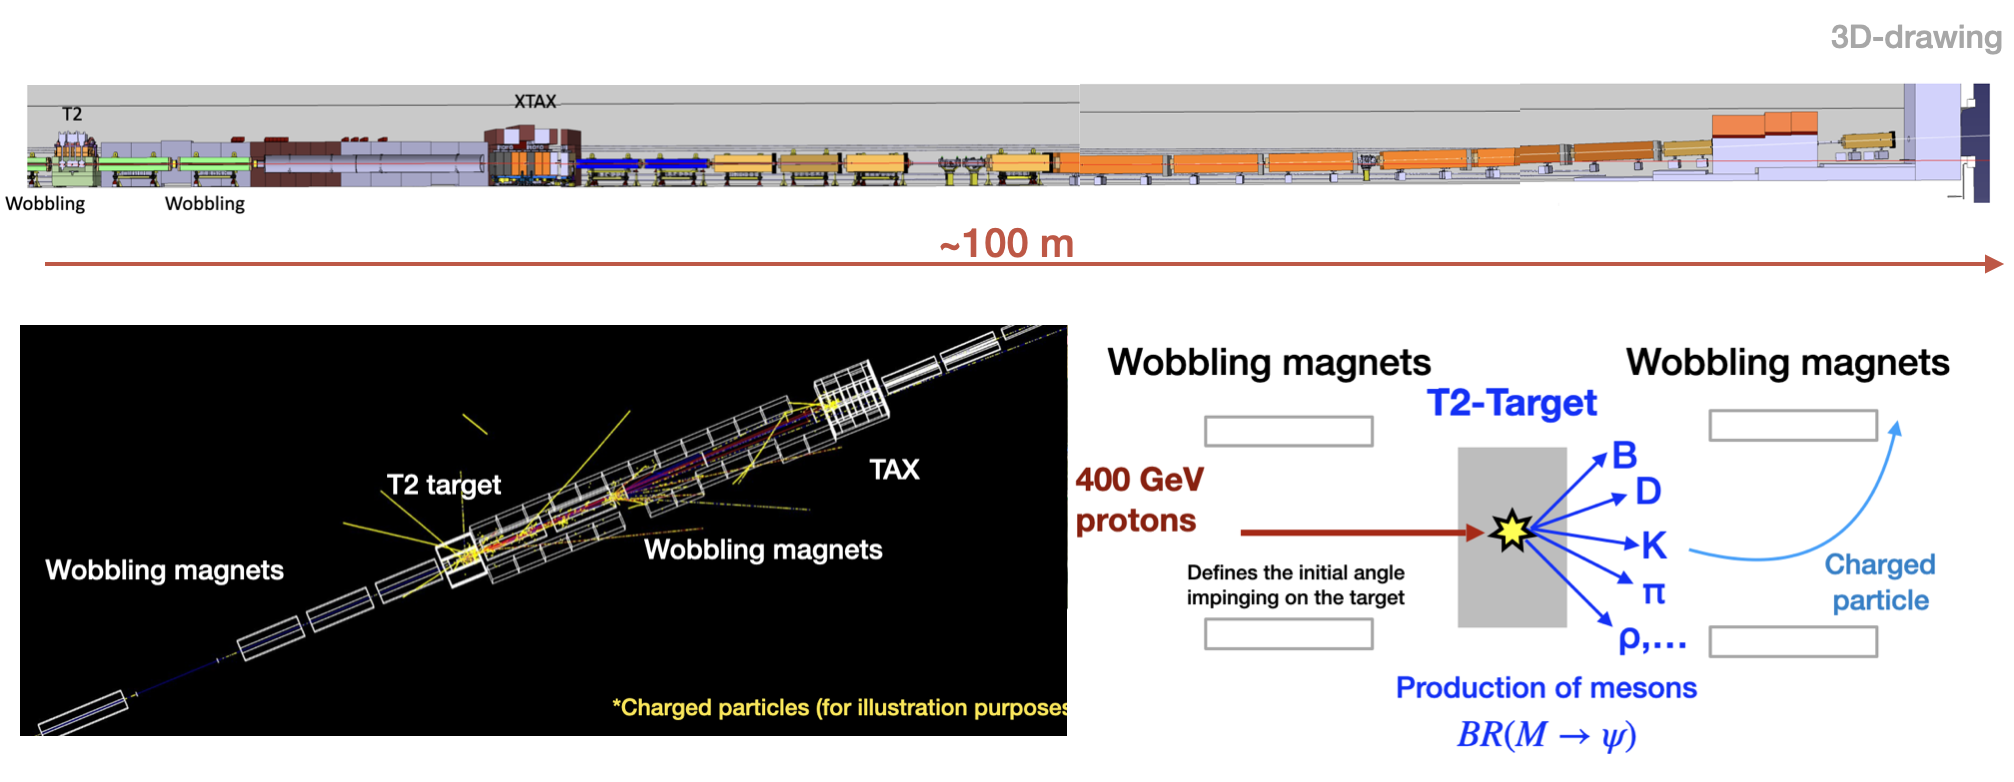
\includegraphics[width=0.95\linewidth]{sections/exp_setup/plots/T2targetComplex.png}
    \caption{Top: 3D model of the T2 target area. Bottom: Schematics of the interaction in T2 for a particular configuration illustrating the production of the mesons that can be a potential source for BSM particles.}
    \label{fig:map_beam}
\end{figure}

The beamlines at the CERN North Area facility are generated by a high-intensity primary proton beam with a momentum of \SI{400}{\GeV/c}, which is extracted from the Super Proton Synchrotron (SPS) \cite{Banerjee:2925964}. This primary beam impinges on each of the three primary targets, namely T2, T4, or T6, to produce secondary particle beams, as illustrated with blue lines in Figure \ref{fig:map_beam}. The different downstream beamlines are designed to transport secondary and tertiary high-energy particle beams, including protons, kaons, pions, muons and electrons, with varying compositions and purities \cite{Banerjee:2925964, gerbershagen2024iii}. The momentum of these beams typically falls within the range of \SI{10} - \SI{400}{\GeV/c}. For the SPS fixed-target experiments in the North Area (SFTPRO), the duty cycle denotes the fraction of time a stable, high-quality proton beam is delivered to the experiments via slow extraction. A typical SFTPRO operational cycle for the \SI{400}{\GeV/c} protons features a \textit{flat-top} duration of approximately 4.8 seconds, during which the beam is slowly extracted \cite{Banerjee:2925964, Velotti:IPAC2019-WEPMP034, Prebibaj:2848908, papotti2023jacow}. This cycle length, which is typically referred to as the spill, is embedded within a longer, repeating sequence of cycles called a supercycle, which can vary in total length depending on the facility's overall scheduling requirements \cite{Banerjee:2925964, Velotti:IPAC2019-WEPMP034, Prebibaj:2848908}.

%\begin{figure}[h]
 %   \centering
  %  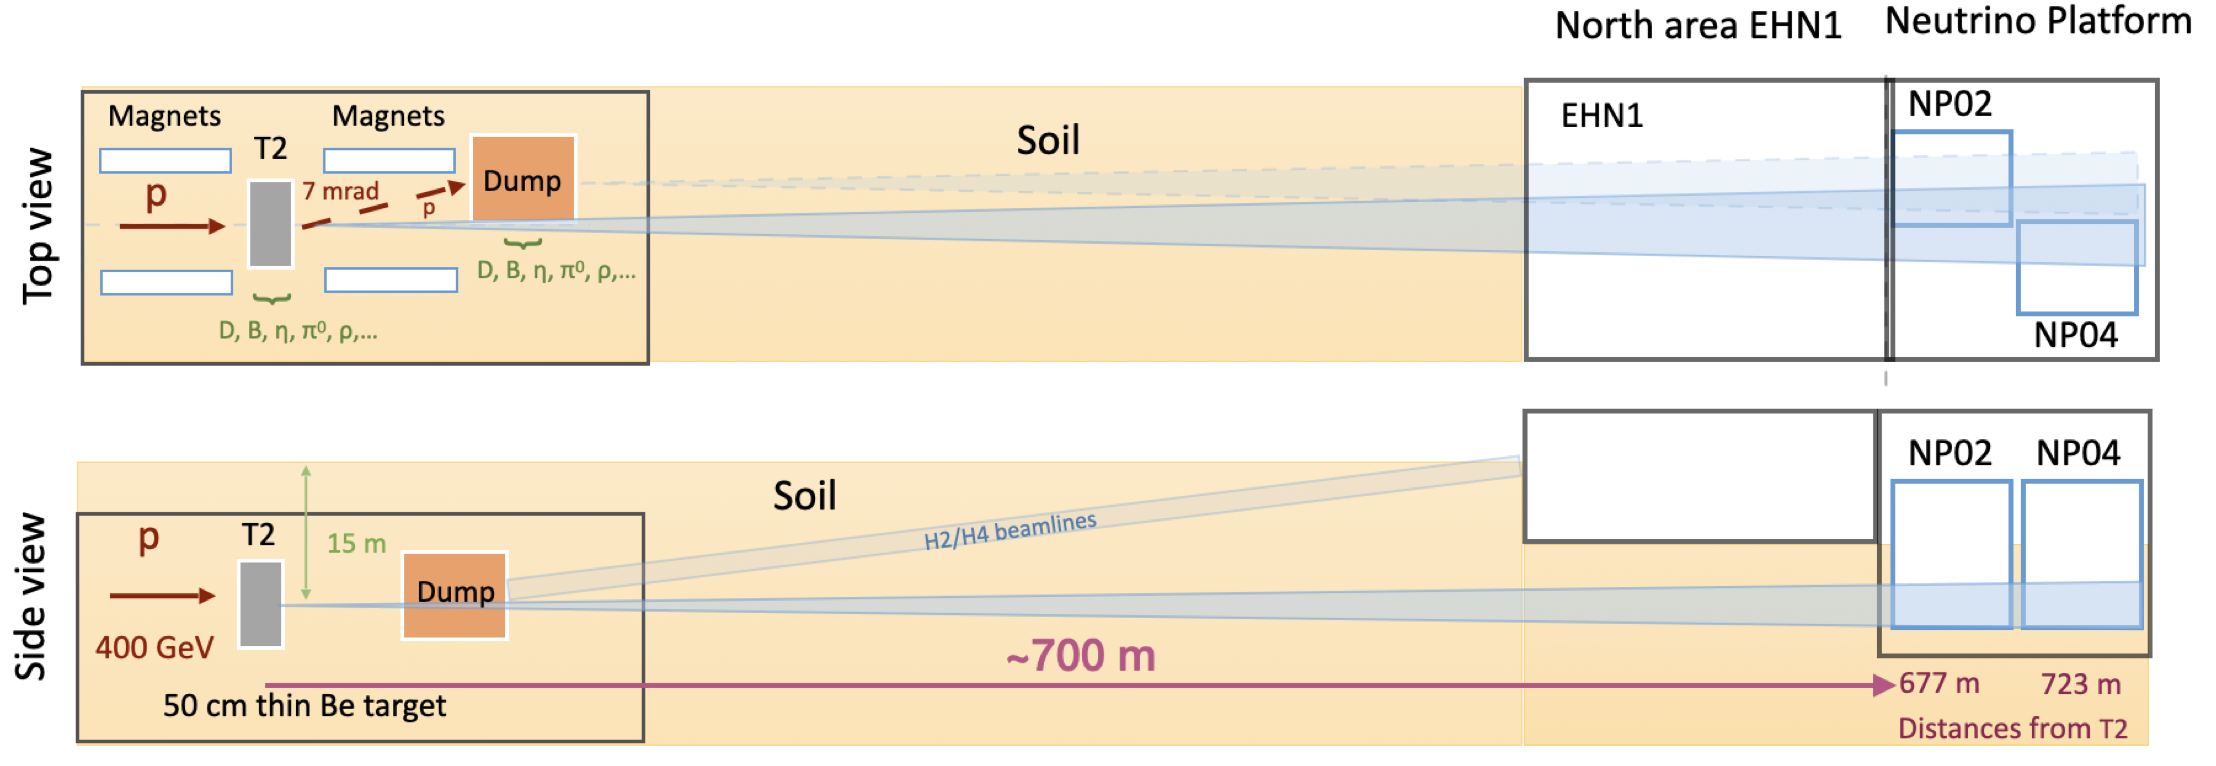
\includegraphics[width=1\linewidth]{sections/data_and_mc/plots/np04_position.png}
   % \caption{Diagram illustrating the generation of secondary particles from the interaction of the primary protons from the SPS an the beryllium T2 target. The ProtoDUNE detectors are exposed to a potential flux of neutral particles from meson decay (see blue area). The relative positioning of the ProtoDUNE detectors from the T2 target location is also remarked \cite{coloma2024new}.}
    %\label{fig:position_detector}
%\end{figure}

 The extracted protons interact with the 50 cm thick T2 beryllium target located approximately 15 meters underground for radiation shielding \cite{coloma2024new} (see the left plot of Figure~\ref{fig:map_beam}). A set of magnets determines the incoming angle of the protons interacting with T2. The remaining protons arising from the target are deviated towards the Target Attenuator for Experiments (TAX) \cite{SBA_TAX_Description_CERN}, an iron structure measuring 3.2 meters in length. The TAX serves as a beam dump, effectively attenuating the remaining protons. The flux of secondary particles emerging from T2 is controlled and shaped by the magnets positioned downstream from the target, {which are called the \it wobbling magnets}. The current of these magnets varies depending on the requirements from the experiments using the H2 and H4 secondary beamlines. This configuration is a crucial parameter in the analysis presented in this work. Depending on the currents applied in the magnets, the secondary particle trajectories deviate and their kinematics differ (this is especially relevant for kaons and charged pions, one of the main sources for the neutrinos). The enabled magnet configuration therefore determines the flux of neutrinos and BSM particles at ProtoDUNE, as shown in Figure~\ref{fig:fluxes_nu_nubar} and explained in detail in section \ref{chap:montecarlo}. It is therefore possible to select a magnet configuration that is most suitable for potential BSM studies \cite{coloma2024new}. Achieving the sensitivity presented in \cite{coloma2024new} requires collecting data at the ProtoDUNE detectors parasitically over several years of SPS beam time whilst developing a complete understanding of the expected signal and background rates for different magnet configurations. The following beam configurations were considered for this study:
 %, combining the ones used in Monte Carlo simulations representing the most extreme cases, and the one settled during the parasitic run:
 %In this work we have compared some of the most relevant wobbling configuration as is computationally demanding simulate all of them. (Not necessary)
\begin{itemize}
    \item \textbf{wNP04}: Configuration used when ProtoDUNE Horizontal Drift was exposed to the dedicated low energy beam produced in H4. This configuration was simulated to compare with the existing PD data. It produces a hadron beam in the secondary beam system. In this configuration the amount of neutrinos from kaon and pion decays is larger as well as the muon flux arriving to the detector.  
    \item \textbf{w133}: Configuration employed to produce an electron beam in the secondary beam lines. Fewer neutrino interactions are expected to be collected with these settings,for which data was collected (see Section 5) but is not used in this analysis due to incomplete reconstruction. 
    \item \textbf{wGIF++}: This configuration is the one used by the Gamma Irradiation Facility, an experiment using the H4 beamline during the data recorded for this study. The GIF++ and wNP04 configurations have identical magnet positioning around the T2 target. They are therefore expected to produce very similar neutrino fluxes. Nevertheless, an important distinction between these two configurations lies in the facilities downstream of the target. In the case of GIF++ a high-intensity muon beam is created after a muon converter from pion decay at the Particle Physics Experiment 124 area. This can be a potential additional source of neutrinos which may arrive to the ProtoDUNEs. This is the configuration used for the data analyzed in this note (see Section 5).
\end{itemize}

%Another aspect relevant for the study, especially for possible beam-related backgrounds affecting the neutrino reconstruction is the position of the ProtoDUNE detectors with respect to the secondary H2, H4 and H6 beamlines. They are located at the end of the lines as illustrated in \ref{fig:beamline}. Therefore, we have analyzed the influence of the activity in the lines due to experiments running in the collected data. The ProtoDUNE Horizontal Drift detector is exclusively exposed to the activity associated with the H4 and H6 beamlines, while ProtoDUNE Vertical Drift is sensitive to both H2 and H4 beamlines, as illustrated in Figure \ref{fig:beamline}. This technical note focuses on the HD.
An important consideration for understanding potential beam-related background is the position of the ProtoDUNE detectors with respect to the secondary H2, H4 and H6 beamlines. Both detectors are exposed to a dedicated extension of the beamlines to inject low-nergy beams in to the ProtoDUNE for the dedicated data taking campaigns (see further details in \cite{Charitonidis:2017omo, Booth:2019brj}. The neutrinos and possible BSM particles, subject of this study, are produced in the targets hundred of meters upstream. Nevertheless, as illustrated in Figure~\ref{fig:beamline}, the ProtoDUNE detectors are located at the end of the secondary beamlines, and therefore are exposed to their activity. We studied if this can be a potential source of background. Due to its location, the ProtoDUNE Horizontal Drift detector is exclusively exposed to the activity associated with the H4 and H6 beamlines, while ProtoDUNE Vertical Drift is sensitive to both H2 and H4 beamlines, as indicated in Figure~\ref{fig:beamline}. This technical note focuses on the PD-HD.

\begin{figure}[ht]
    \centering
    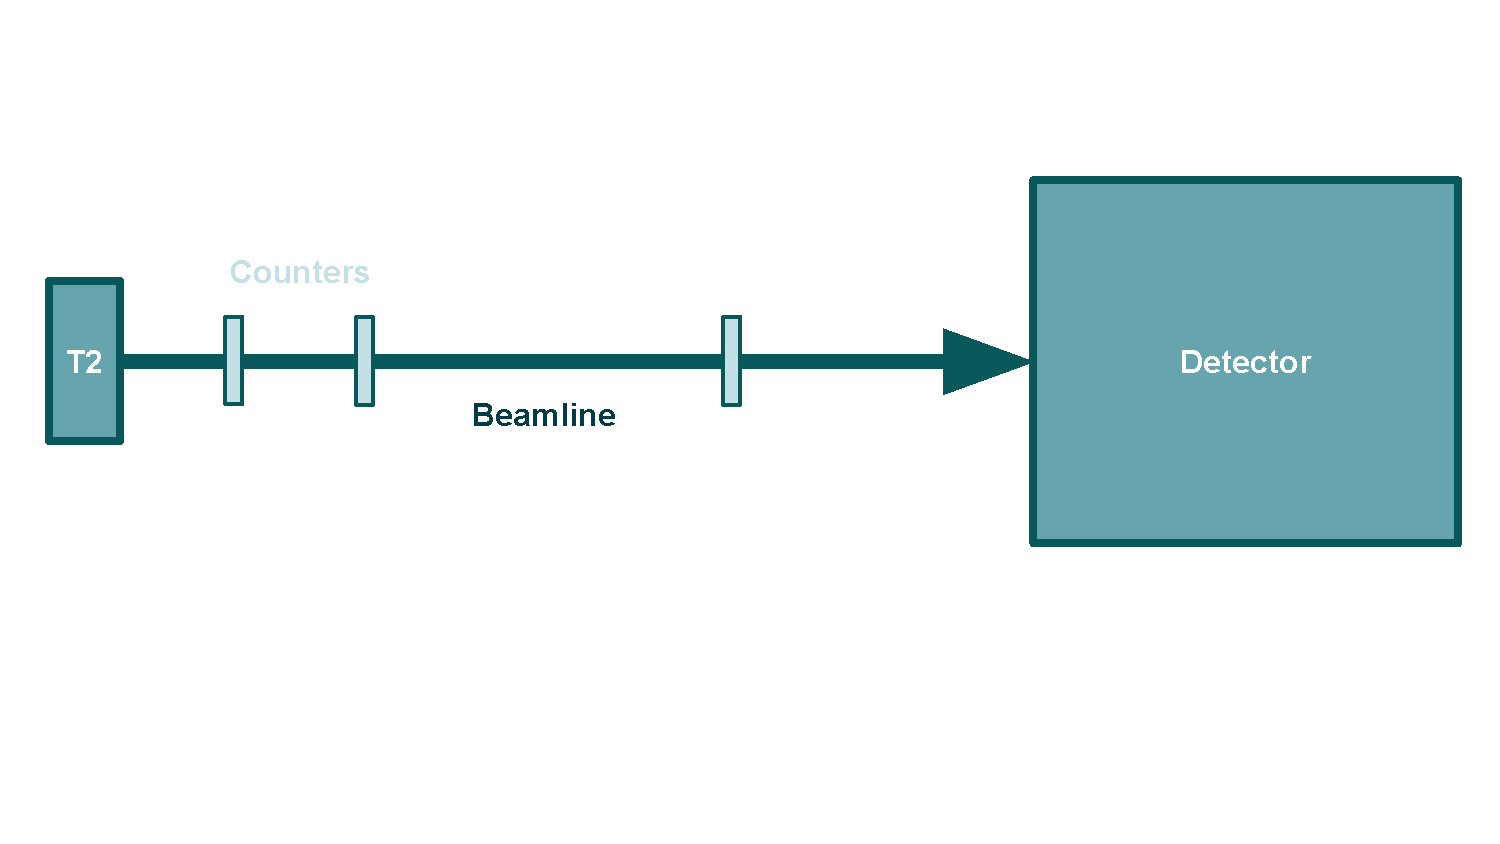
\includegraphics[width=0.8\linewidth]{sections/exp_setup/plots/schemeBeamline.pdf}
    % 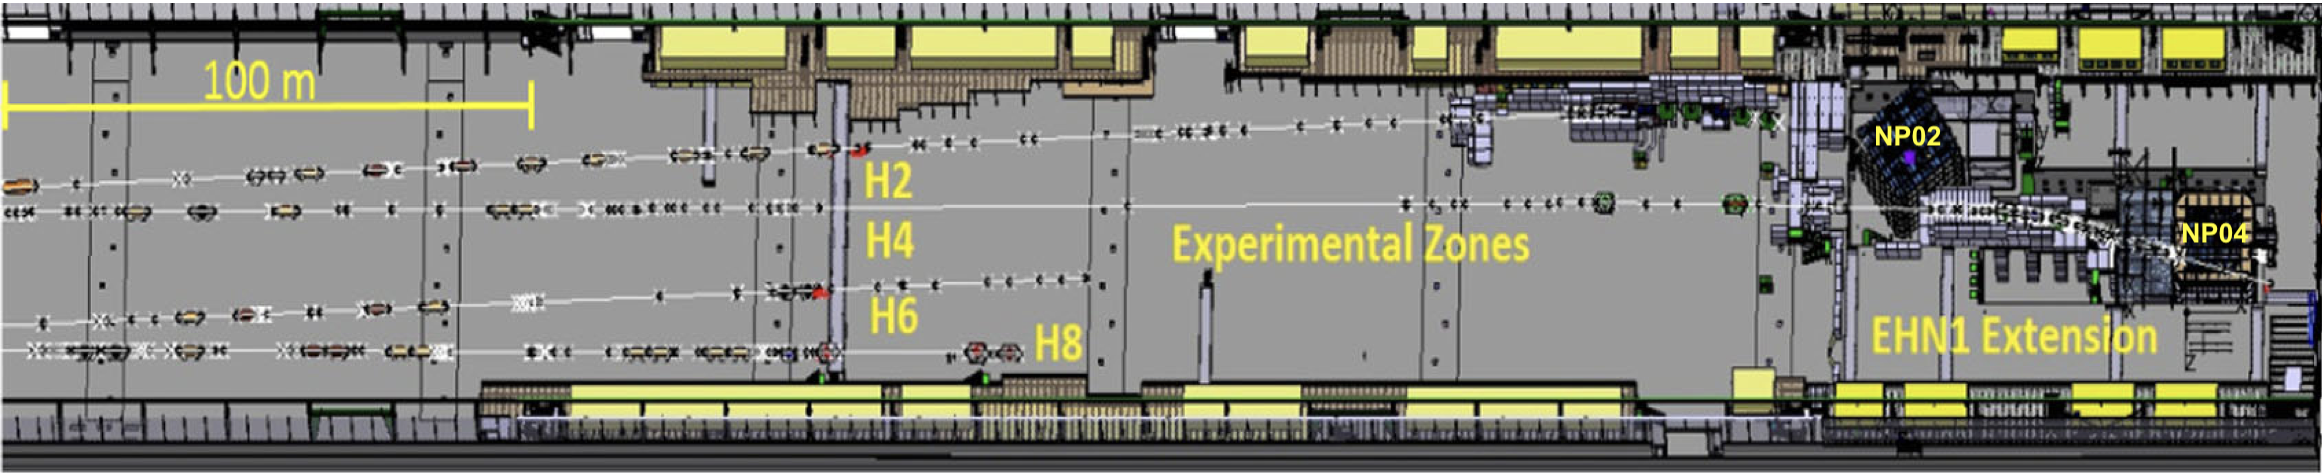
\includegraphics[width=1\linewidth]{sections/exp_setup/plots/Beamlines.png}
    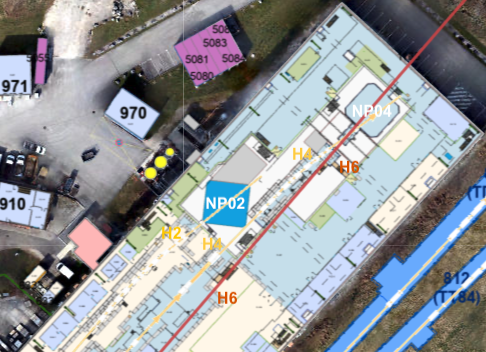
\includegraphics[width=0.75\linewidth]{sections/exp_setup/plots/HBeamlines.png}
    \caption{Schematic representation of a set of scintillation counters strategically positioned along the beamline in between the T2 target and the detector (top), and a layout of the EHN1 downstream hall (bottom). The extension part for the hall in the Neutrino Platform is shown on the right part. PD-VD is exposed to H2 and H4 beamline activity, while PD-HD is exposed to H4 and H6.}
    \label{fig:beamline}
\end{figure}

% During the runs analyzed in this note, recorded parasitically, we did not access the information of all available scintillator counters. Its placement along the line depend on the experimental users and we did not obtain such information during data taking. Hence, the farthest downstream monitors, located closest to the detector, were exclusively analyzed to seek for specific correlations between the detector and the beamline activities. Preliminary results indicate such a good correlation between the most downstream scintillator counters placed along the H4 and H6 beamlines and the Trigger Primitives collected in ProtoDUNE for the GIF++ magnet configuration (see section \ref{chap:anaBeamMonitoring}). Future studies in the coming PD-VD run foresee a dedicated study on the correlation between the activity in the secondary lines and the ProtoDUNE recorded events.

%The primary application that provides the CERN North Area experiments with beam information is known as \href{http://timber.cern.ch}{TIMBER}. It offers access to CERN Accelerator Logging Service data. From TIMBER, one extracts a time flag per spill, which indicates the beginning and end of the spill, as well as the protons on target (PoT). For this study, a favorable spill was deemed to be one that exceeded the PoT threshold of $10^{12}$. Failing this, the spill was disregarded. In this manner, one ensures to tag the detector activity based on the spill modes, which are referred to in this note as \textit{spill on} and \textit{spill off}. In this note, \textit{spill off} denotes time between and during spills which have less than $10^{12}$ PoT.

% During the runs analyzed in this note, recorded parasitically, we did not access the information of all available scintillator counters. Its placement along the line depend on the experimental users and we did not obtain such information during data taking. Hence, the farthest downstream monitors, located closest to the detector, were exclusively analyzed to seek for specific correlations between the detector and the beamline activities. Preliminary results indicate such a good correlation between the most downstream scintillator counters placed along the H4 and H6 beamlines and the Trigger Primitives collected in ProtoDUNE for the GIF++ magnet configuration (see section \ref{chap:anaBeamMonitoring}). Future studies in the coming PD-VD run foresee a dedicated study on the correlation between the activity in the secondary lines and the ProtoDUNE recorded events. %Unfortunately, during the data-taking campaign, the scintillation counters were not necessarily in place. Consequently, the runs presented in section \ref{chap:anaBeamMonitoring} are those which exhibit specific correlations. At present, this analysis is conducted for PD-VD under different beam configurations, in collaboration with the H2 and H4 beamline managers, ensuring that the scintillators are properly in place.

 %A first attempt was done last year before the end of the SPS year although we had limited time for such tests. Preliminary results indicate such a good correlation between the most downstream scintillator counters placed along the H4 and H6 beamlines and the Trigger Primitives collected in ProtoDUNE for the GIF++ magnet configuration. 
% However, for further conclusions dedicated longer runs in different configurations will be needed. 

%To evaluate the impact during the PD-VD posterior run, a set of scintillation counters are placed along the H2 or H4 beamlines. The number of counts in each scintillator  would be eventually compared with the detector activity for the sake of linear correlations. The diverse range of scintillators can be accessed through TIMBER. 

\subsection{The ProtoDUNE detector} \label{chap:protodune_det}

The ProtoDUNE Horizontal Drift detector is a liquid argon TPC (LArTPC) installed at the CERN Neutrino Platform and is an iteration on the original ProtoDUNE Single Phase detector~\cite{ProtoDUNESP_2020}. %It is a full-scale prototype of one of the Deep Underground Neutrino Experiment (DUNE) \cite{DUNE:2020lwj} far detector modules. 
It serves as a testbed for detector elements encompassing electronics, the DAQ system, data management, and calibration and monitoring systems. The PD-HD is situated 720 meters downstream from the T2 target.

\begin{figure}[h!]
    \centering
    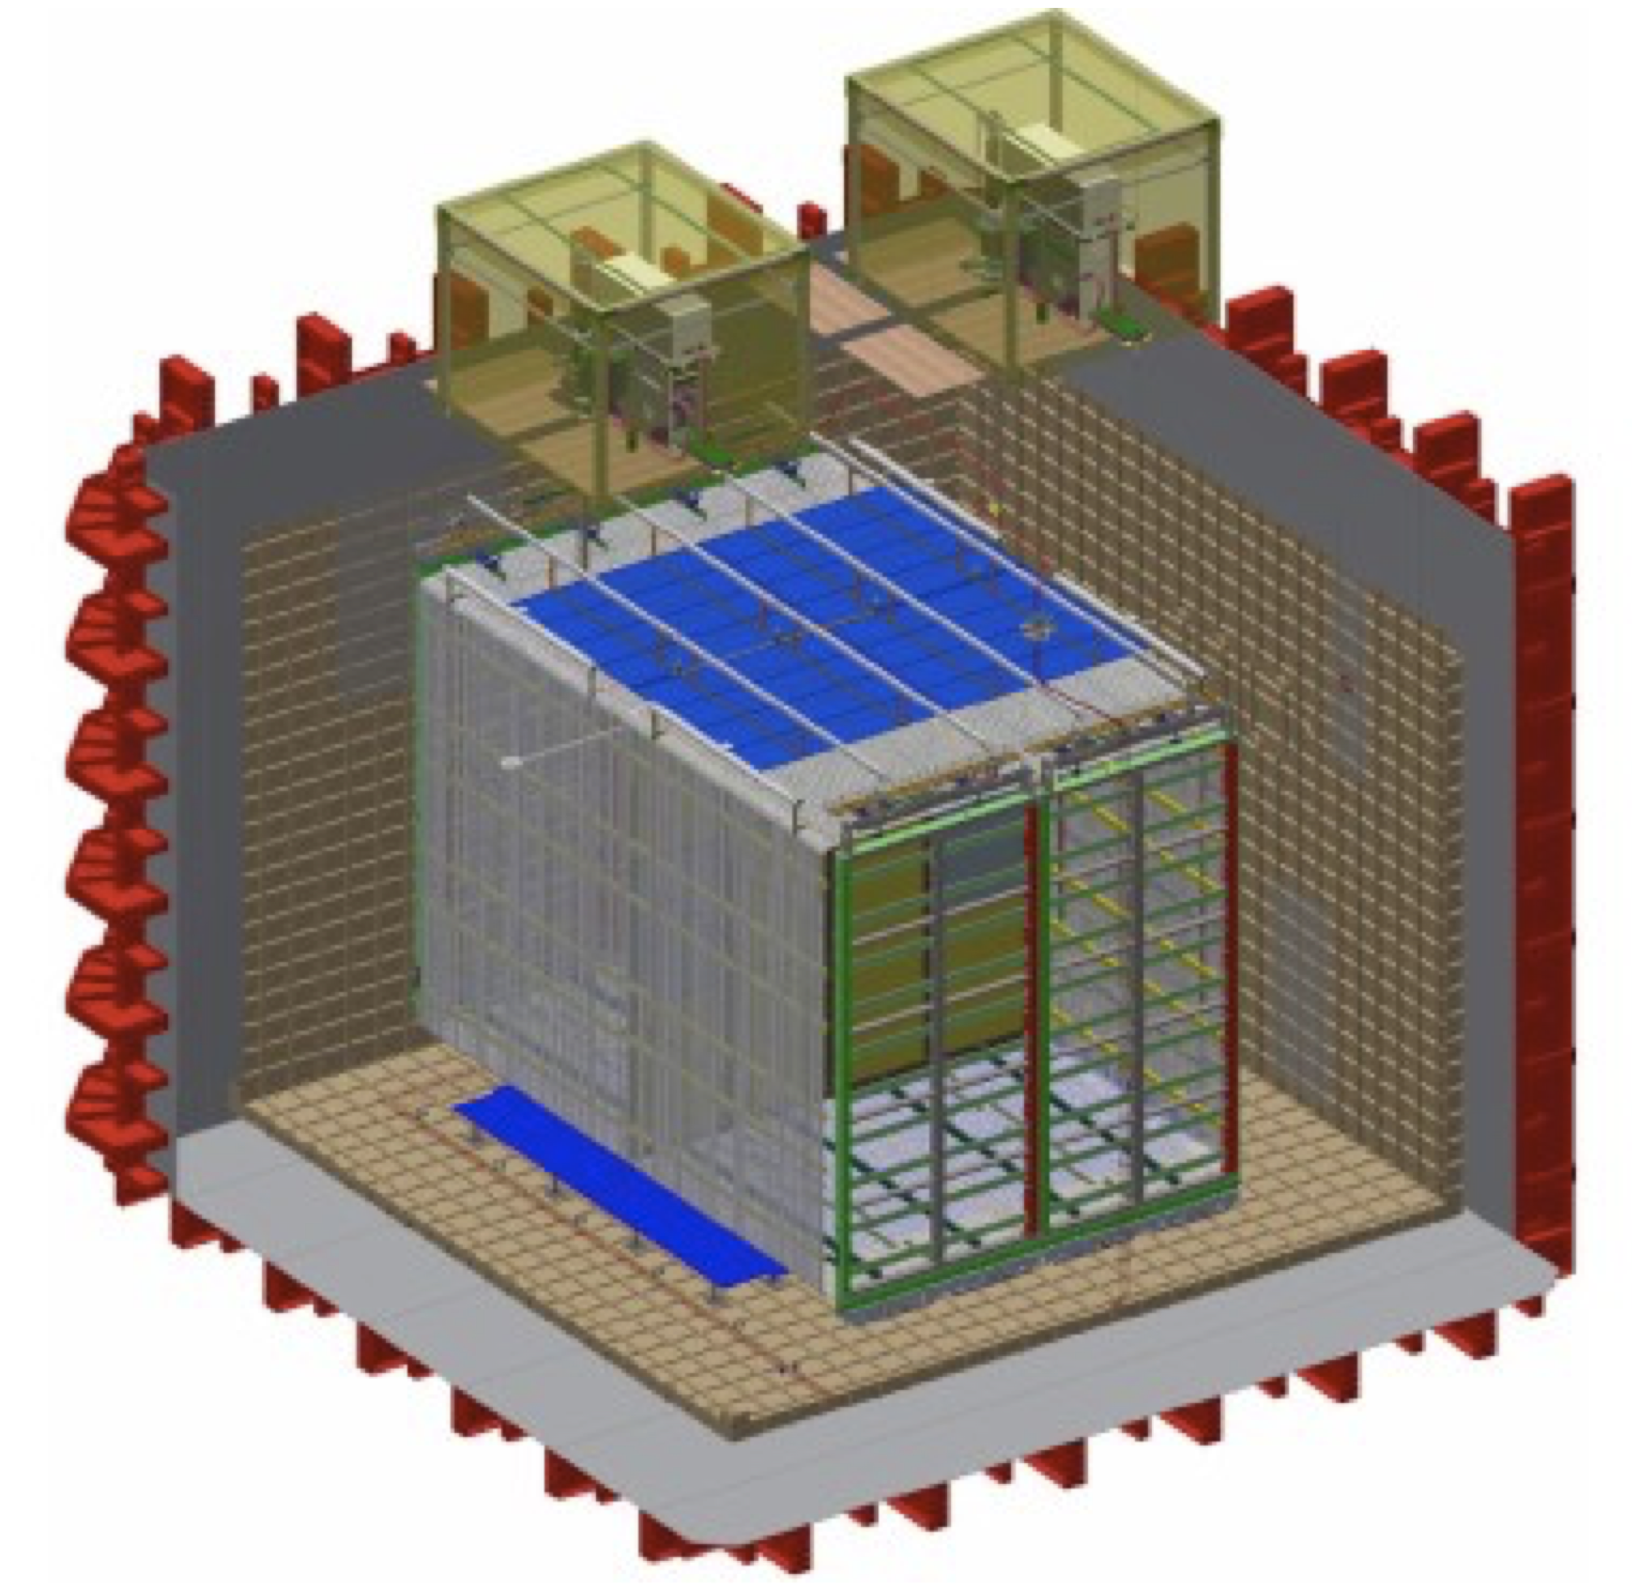
\includegraphics[width=0.75\linewidth]{sections/exp_setup/plots/3d_model_pdhd.png}
    \caption{A 3D model of the PD-HD geometry, including the cryostat and the internal active volume.}
    \label{fig:3d_model}
\end{figure}

The detector is embedded in a cryostat with internal dimensions of 8.5 m width and length and 7.9 m height, as illustrated in Figure \ref{fig:3d_model}. The active volume is divided in two sections by the central cathode and extends for 3.6 m to the anode planes which are made of 2 Anode Plane Assembly units (APAs) per side, for a total active length of 4.6 m and a height of 6.1 m, respectively, corresponding to approximately 250 tons of liquid argon. In the ProtoDUNE coordinate system, the X component is along the drift direction, the Y component is the vertical direction, and the Z component corresponds to the beam direction, parallel to the cathode. Its origin is located at the lower, most upstream corner of the central cathode. The detector coordinate system and geometry of PD-HD is illustrated in Figure \ref{fig:top_view_scheme}.

%The Anode Plane Assembly (APA) is the fundamental unit used to extract signals from the detector. 
The APA is composed of planes of wires that extract signals from the detector. Each APA comprises a total of 2560 active wires, with each wire connected to an individual readout channel. The wire pitch is 4.79 mm for the collection plane and 4.67 mm for both induction planes. The three wire planes—U and V (induction) and X (collection)—are arranged in layers on each side of the APA, with carefully chosen relative angles to minimize ambiguities in event reconstruction.

The wire readout is sampled at an interval of 512 ns, resulting in a sample rate of approximately 2 MHz. In contrast, the DUNE timing system (DTS) is based on the Photon Detection System (PDS) clock, which has a higher sampling rate of 62.5 MHz, corresponding to a time interval between the ticks of 16 ns.

Channels numbered from 0 to 799 and from 800 to 1599 make respectively the U and V induction planes, which are transparent to drifting electrons and produce a bipolar signal in the wires. These planes cover both sides of the APA by wrapping around the structure at a turning angle of 35.7 degrees relative to the vertical axis. The remaining 960 wires form the innermost readout plane, the collection plane, commonly referred to as X. This plane finally collects the electrons, thus resulting in a unipolar signal. The collection wires are perfectly vertical and cover one single side of the APA, providing an unambiguous indication of the APA's side where the event occurred, in contrast to the U and V planes. 

%A schematic layout of the detector is shown in Figure~\ref{fig:top_view_scheme}.

\begin{figure}[h!]
    \centering
    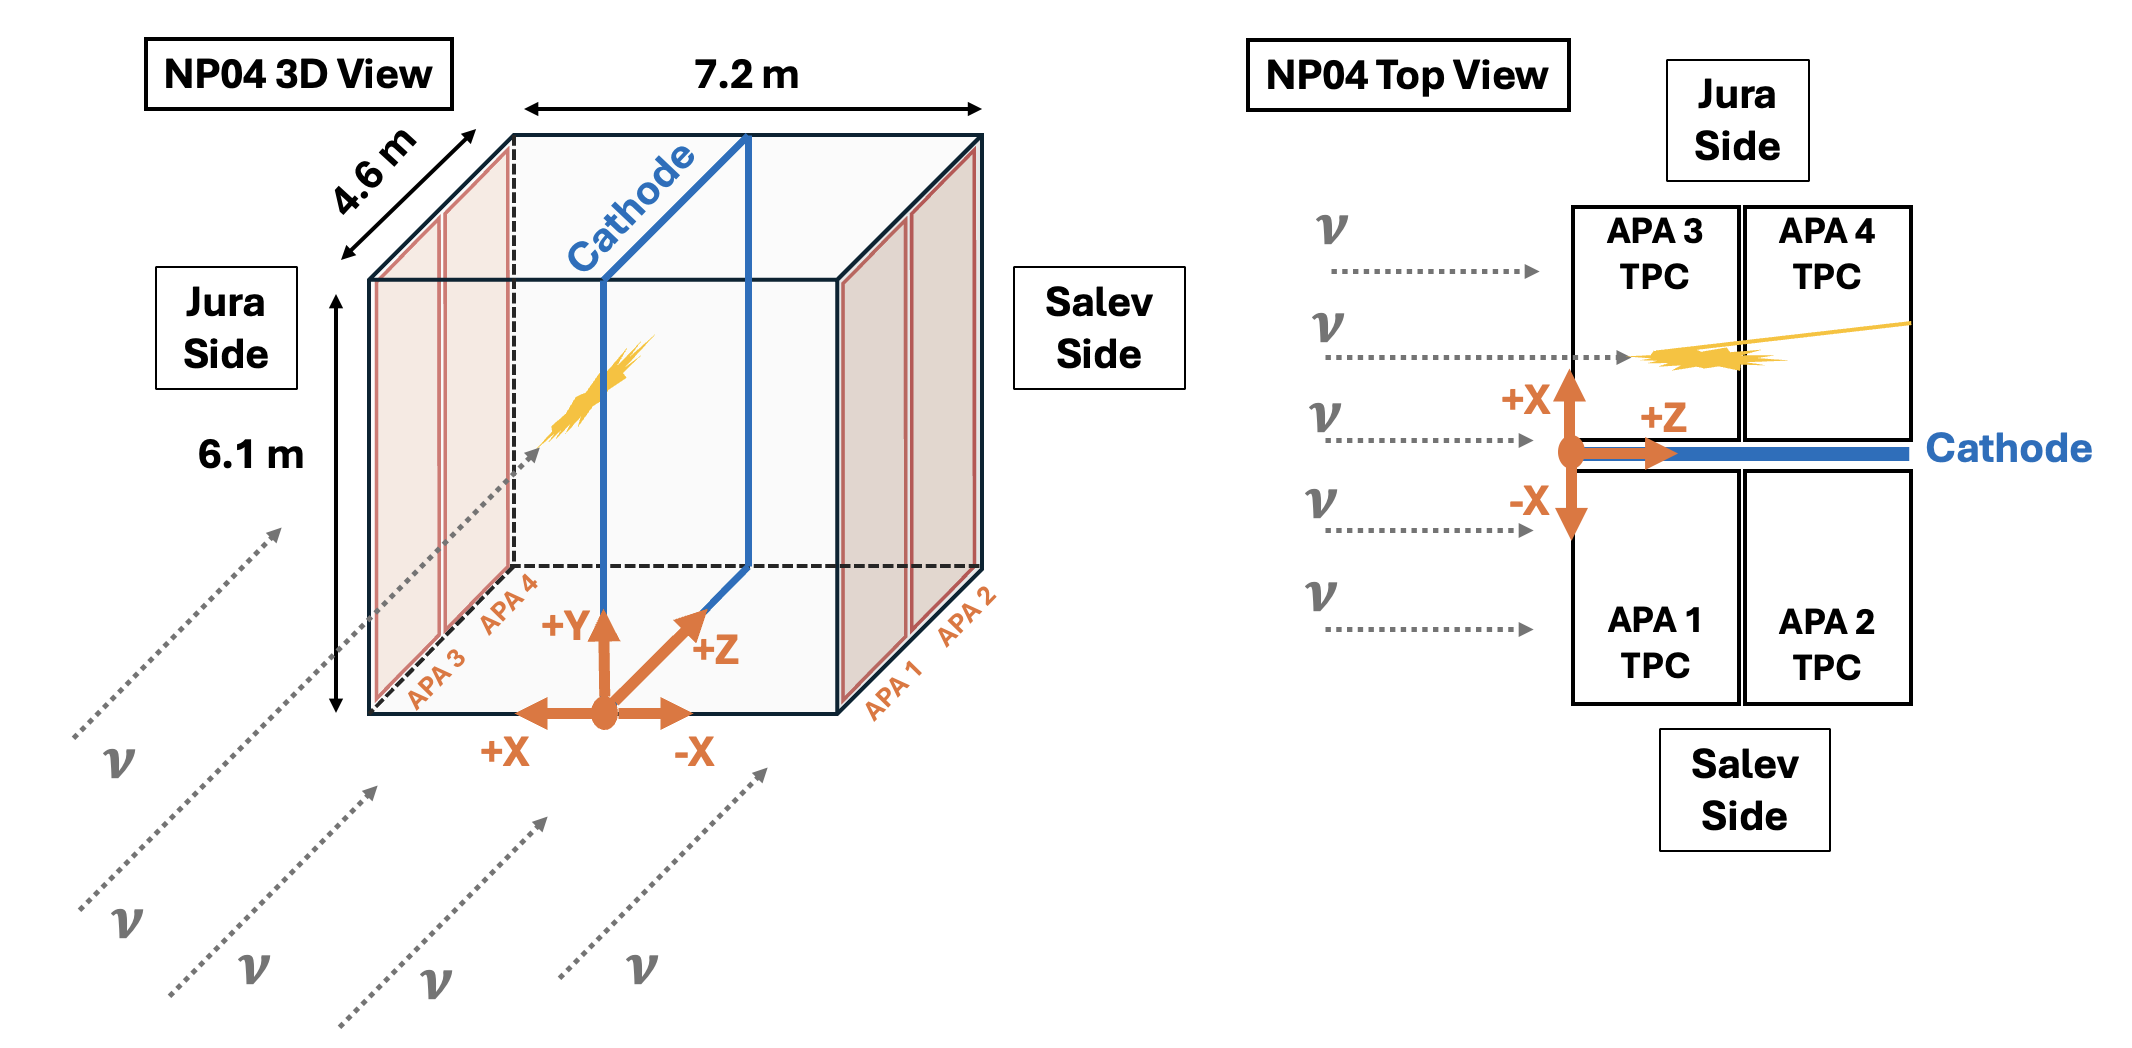
\includegraphics[width=0.95\linewidth]{sections/exp_setup/plots/NP04_GeometryIllustration_3D_and_Top.png}
    \caption{Two views of the PD-HD geometry. The left illustration shows the three-dimensional geometry of PD-HD, including the dimensions of the active TPC and the locations of the four APAs. A central cathode separates the drift volumes. The right diagram shows the geometry of PD-HD from the top view. Both figures illustrate the detector coordinate system used in the later analysis. The direction of the incoming neutrinos from the T2 target 720~m upstream is illustrated. All the neutrinos are traveling parallel to the central cathode of ProtoDUNE, leading to energy deposits upon interaction within the TPC that are confined to a narrow region in the x-direction.}
    \label{fig:top_view_scheme}
\end{figure}

During the operations, the collection plane of one of the APAs (APA 1) was not properly working, making the corresponding active volume harder to reconstruct. Having the full length of the detector available is a major advantage because the interactions that happen in the most downstream parts of the volume are likely to deposit energy outside the active volume and therefore provide less information.
